\chapter{Comparación entre versiones de Python \emph{free-threaded}}
\label{chap:versiones}

El capítulo anterior muestra que, en la campaña principal con Python~3.15t, el
modo~3 de OMP4Py produce tiempos competitivos y escala en EP y FT, mientras que
CG, IS y MG presentan límites de paralelización. Este capítulo estudia si ese
comportamiento depende de la versión concreta del intérprete
\emph{free-threaded}, y recorre para ello los cuatro modos de ejecución. La
respuesta tiene dos caras. En los modos interpretados la versión importa mucho,
porque la primera build \emph{free-threaded}, la 3.13t, escala bastante peor al
aumentar los hilos. En los modos compilados esa diferencia desaparece. Por eso el
capítulo arranca por los modos interpretados, donde el efecto es mayor, y después
comprueba que el tipado lo anula.

La comparación cubre Python~3.13.13t, Python~3.14.4t y Python~3.15.0b1t,
todas compiladas con el GIL desactivado. Las campañas finales se ejecutaron con
el mismo código fuente, la misma infraestructura de Slurm, las mismas clases y
el mismo rango de hilos. Además, se eliminaron las variables de afinidad de
OpenMP que habían producido resultados preliminares no representativos. Por
tanto, la variable experimental de este capítulo es la versión del intérprete y
su ABI \emph{free-threaded}.


\section{Diseño de la campaña}
\label{sec:versiones-diseno}

La campaña de comparación entre versiones se diseñó como un subconjunto de la
campaña principal, pero manteniendo todas las potencias de dos hasta 32~hilos.
Se ejecutaron CG, EP, FT, IS y MG con los recuentos de hilos 1, 2, 4, 8, 16
y~32. Los modos compilados~2 y~3 se midieron en las clases~S y~W, y los modos
interpretados~0 y~1 en la clase~S, el único tamaño donde el código no compilado
termina en un tiempo razonable. La clase~S se ejecutó con cinco repeticiones por
combinación y la clase~W con tres. La campaña completa contiene
2340~ejecuciones, 1440 en los modos compilados y 900 en los interpretados, y
todas finalizaron con verificación \texttt{SUCCESSFUL}.

No se incluyó la clase~A porque el coste habría multiplicado el uso del cluster.
La clase~A ya se evaluó con Python~3.15t en la campaña principal, y esta campaña
se centra en comprobar si las tendencias de S y W cambian al modificar el
intérprete. Como en el resto de la memoria, se usa el mejor tiempo NAS entre las
repeticiones válidas.


\section{Efecto de la versión en los modos interpretados}
\label{sec:versiones-interpretado}

La comparación empieza por los modos~0 y~1, donde los kernels se ejecutan como
Python interpretado y es el propio intérprete el que realiza el trabajo. La
Tabla~\ref{tab:versiones-interpretado-completo} recoge el tiempo NAS de los cinco
benchmarks en los dos modos interpretados, para las tres versiones y todos los
recuentos de hilos, y la Figura~\ref{fig:versiones-interpretado}, al final de la
sección, lo muestra de forma gráfica.

\begin{table}[H]
\centering
\scriptsize
\renewcommand{\arraystretch}{0.92}
\adjustbox{max width=\textwidth}{%
\begin{tabular}{llrrrrrr}
\hline
 & & \multicolumn{3}{c}{Modo 0} & \multicolumn{3}{c}{Modo 1} \\
Bench. & Hilos & 3.13t & 3.14t & 3.15t & 3.13t & 3.14t & 3.15t \\
\hline
CG & 1 & 18.35 & 18.21 & 18.24 & 18.33 & 18.15 & 18.28 \\
 & 2 & 18.07 & 14.85 & 14.28 & 18.46 & 15.26 & 14.77 \\
 & 4 & 18.30 & 10.23 & 11.12 & 17.79 & 10.31 & 10.92 \\
 & 8 & 31.95 & 12.60 & 12.96 & 32.31 & 12.36 & 12.61 \\
 & 16 & 90.49 & 14.71 & 14.72 & 92.82 & 14.15 & 14.57 \\
 & 32 & 115.78 & 22.36 & 24.15 & 100.69 & 16.75 & 16.61 \\
\hline
EP & 1 & 59.56 & 52.33 & 50.88 & 60.16 & 53.68 & 52.02 \\
 & 2 & 29.73 & 26.31 & 25.88 & 30.67 & 27.44 & 26.53 \\
 & 4 & 15.26 & 13.27 & 12.96 & 15.56 & 13.90 & 13.45 \\
 & 8 & 7.57 & 6.72 & 6.52 & 7.86 & 7.11 & 6.71 \\
 & 16 & 4.08 & 5.13 & 3.39 & 3.87 & 4.10 & 3.35 \\
 & 32 & 2.10 & 3.58 & 1.74 & 2.24 & 3.50 & 2.05 \\
\hline
FT & 1 & 42.88 & 47.50 & 39.32 & 39.97 & 47.54 & 39.21 \\
 & 2 & 25.17 & 25.98 & 22.65 & 24.92 & 25.98 & 22.85 \\
 & 4 & 15.12 & 14.69 & 12.87 & 15.37 & 14.49 & 12.90 \\
 & 8 & 10.70 & 9.35 & 8.34 & 10.92 & 9.43 & 8.27 \\
 & 16 & 14.38 & 8.18 & 7.56 & 15.15 & 8.17 & 7.55 \\
 & 32 & 17.85 & 8.63 & 8.16 & 18.21 & 8.61 & 8.17 \\
\hline
IS & 1 & 0.33 & 0.32 & 0.33 & 0.33 & 0.32 & 0.33 \\
 & 2 & 0.28 & 0.22 & 0.22 & 0.29 & 0.22 & 0.22 \\
 & 4 & 0.25 & 0.15 & 0.15 & 0.23 & 0.15 & 0.15 \\
 & 8 & 0.39 & 0.17 & 0.19 & 0.39 & 0.17 & 0.19 \\
 & 16 & 1.01 & 0.24 & 0.25 & 1.02 & 0.24 & 0.25 \\
 & 32 & 1.23 & 0.31 & 0.32 & 1.26 & 0.32 & 0.33 \\
\hline
MG & 1 & 3.69 & 3.70 & 3.80 & 3.69 & 3.67 & 3.80 \\
 & 2 & 3.13 & 2.38 & 2.52 & 3.04 & 2.29 & 2.47 \\
 & 4 & 2.75 & 1.52 & 1.63 & 2.73 & 1.53 & 1.62 \\
 & 8 & 3.32 & 1.26 & 1.32 & 3.16 & 1.27 & 1.29 \\
 & 16 & 8.63 & 1.28 & 1.30 & 8.54 & 1.30 & 1.32 \\
 & 32 & 10.65 & 1.43 & 1.45 & 10.62 & 1.42 & 1.45 \\
\hline
\end{tabular}
}
\caption{Tiempo NAS por número de hilos en los modos interpretados~0 y~1,
clase~S, para Python~3.13t, 3.14t y 3.15t. Tiempos en segundos. Al crecer el
número de hilos, Python~3.13t se degrada mucho más que 3.14t y 3.15t en CG, FT,
IS y MG. EP, \emph{embarrassingly parallel}, es la excepción.}
\label{tab:versiones-interpretado-completo}
\end{table}


Con un solo hilo, CG, IS y MG quedan casi idénticos entre versiones, porque su
cómputo se apoya en NumPy y la ruta caliente corre en C. Los que se separan son
EP y FT, los dos kernels con más trabajo en el propio intérprete. En EP,
Python~3.13t resulta entre un 12\% y un 17\% más lento que 3.14t y 3.15t,
coherente con que la 3.13t desactivara el intérprete especializador por no ser
todavía seguro sin GIL, función que 3.14t recuperó. En FT el margen es aún mayor,
en torno al 20\%, y con otro orden, porque la más lenta es 3.14t.

El cuadro cambia por completo al aumentar el número de hilos
(Figura~\ref{fig:versiones-interpretado}). En CG, FT, IS y MG, Python~3.13t se
degrada mucho más que 3.14t y 3.15t, y la brecha crece con cada duplicación de
hilos. CG en modo~1 pasa de 18.3~s con un hilo, donde las tres versiones
coinciden, a 100.7~s con 32~hilos en 3.13t frente a 16.6~s en 3.15t, seis veces
más. MG llega a ser siete veces más lento en 3.13t a 32~hilos (10.6~s frente a
1.4~s), IS unas cuatro veces y FT algo más del doble. Con un hilo la diferencia no
existe, con 8~hilos ya es de dos a tres veces, y con 32 alcanza de cuatro a siete
veces. Es un efecto sistemático, no ruido, porque se repite en los dos modos
interpretados y en las cinco repeticiones de cada punto.

EP es la única excepción. Al ser \emph{embarrassingly parallel}, sus hilos apenas
comparten estado, así que no sufre ese coste y 3.13t escala con normalidad. Ahí
el único matiz es una ligera regresión de 3.14t a 16 y 32~hilos, que 3.15t
corrige, de modo que 3.15t vuelve a ser la versión más rápida.

La causa está en el coste de coordinación del intérprete sin GIL. Cuando el bucle
caliente manipula objetos Python desde muchos hilos, la primera build
\emph{free-threaded} paga un sobrecoste alto de gestión de referencias y
contención de memoria que 3.14t y 3.15t redujeron. EP no lo nota porque casi no
comparte datos entre hilos. Este es, con diferencia, el mayor efecto de versión
de todo el estudio, y vive por entero en la ejecución interpretada. La sección
siguiente comprueba que, al activar el tipado de los modos compilados, esta
diferencia desaparece.

\begin{figure}[tbp]
\centering
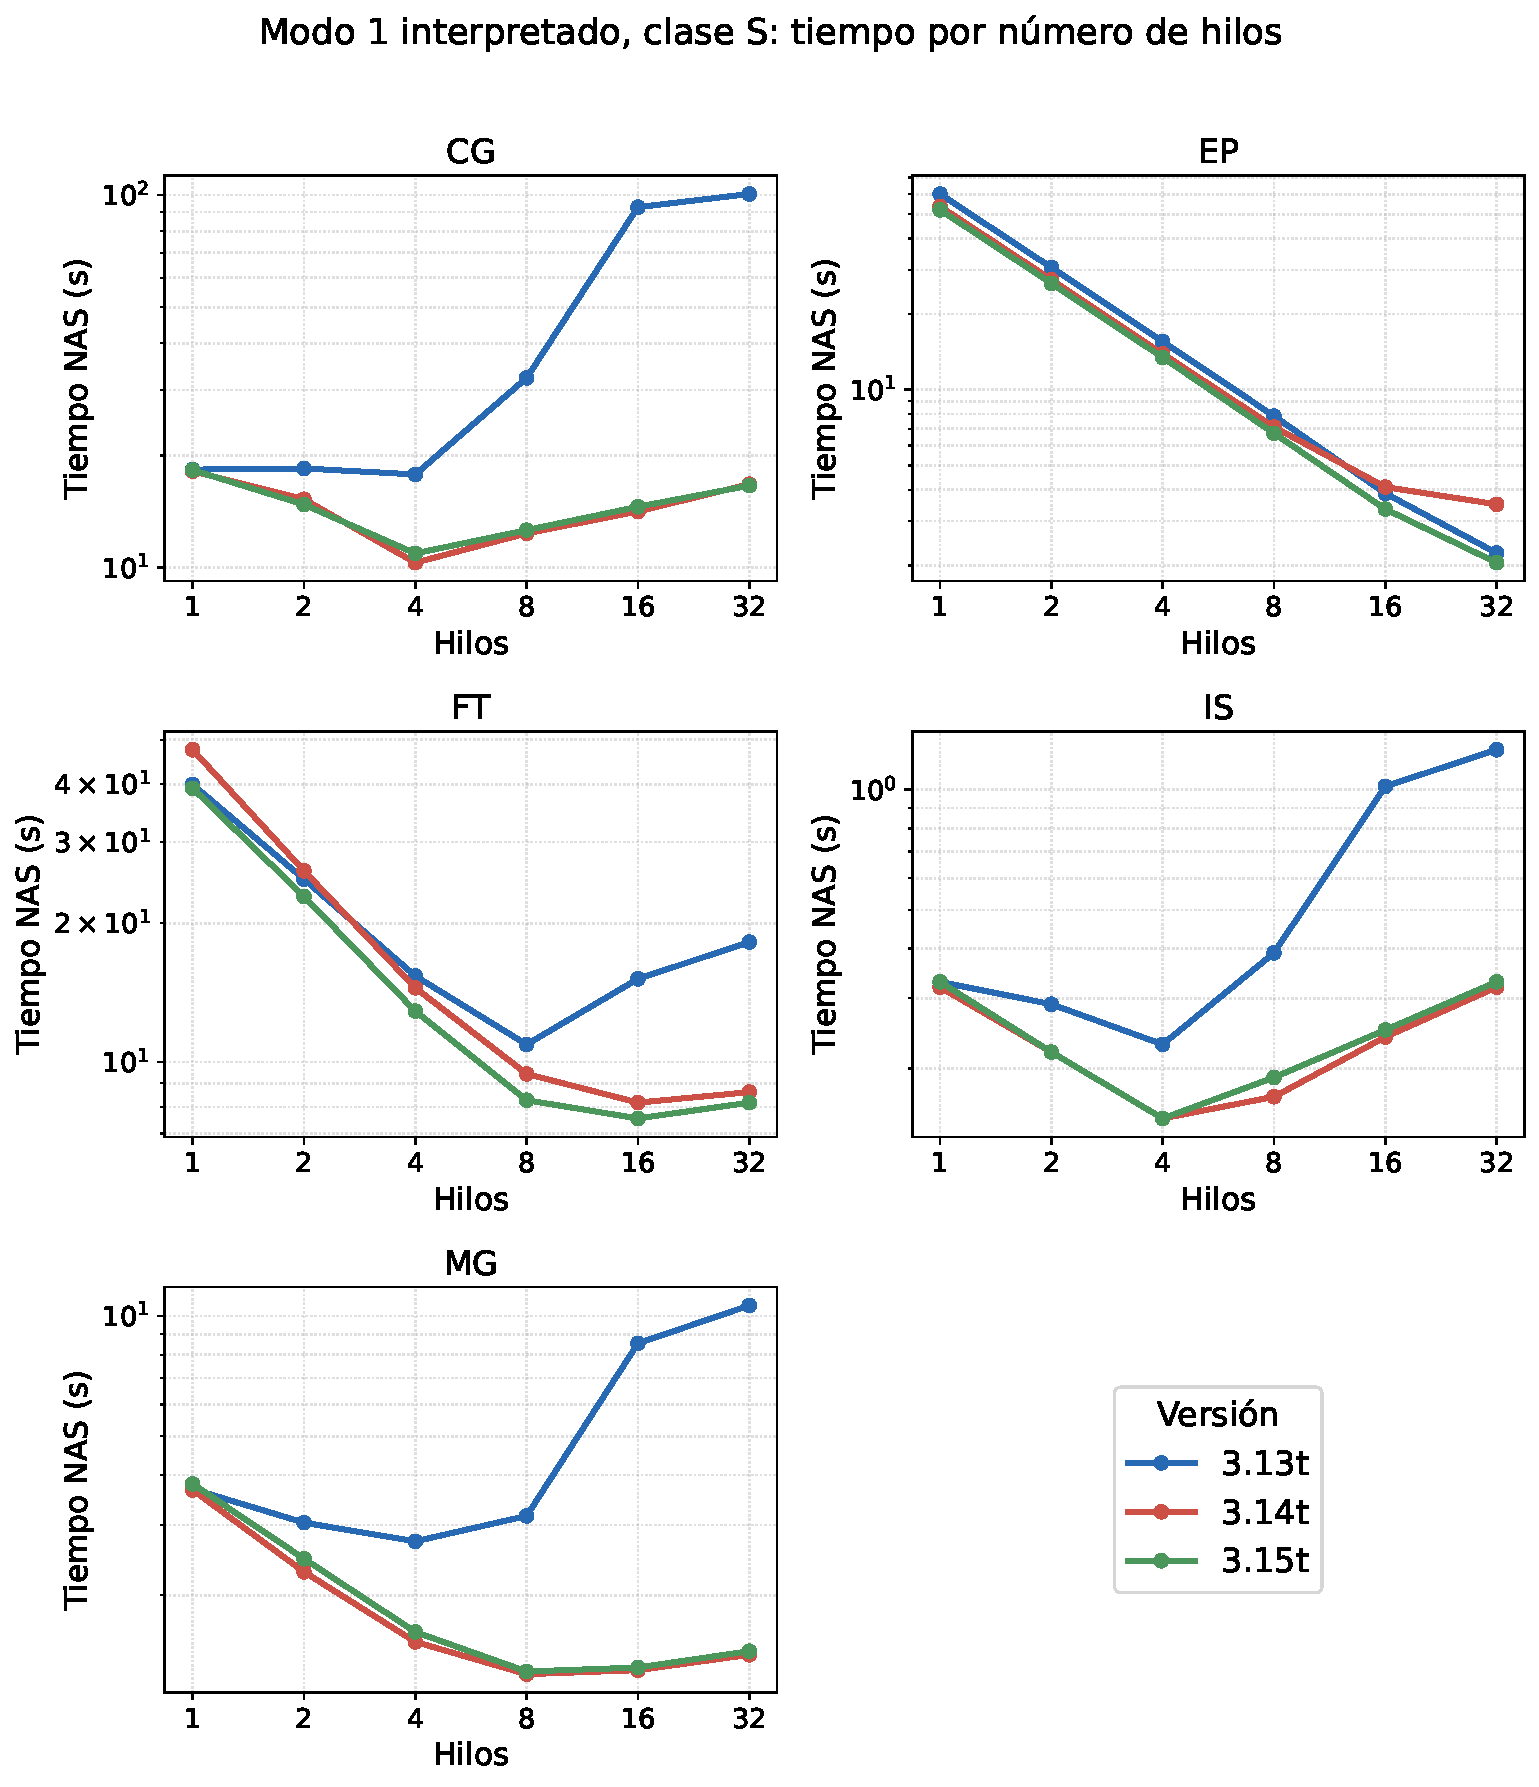
\includegraphics[width=0.92\textwidth]{imagenes/versiones/interpretado_tiempos_versiones}
\caption{Tiempo NAS por número de hilos en modo~1 interpretado, clase~S, para
Python~3.13t, 3.14t y 3.15t. En CG, FT, IS y MG la 3.13t se dispara al aumentar
los hilos, mientras que EP, \emph{embarrassingly parallel}, mantiene las tres
versiones juntas.}
\label{fig:versiones-interpretado}
\end{figure}

\newpage

\section{El tipado neutraliza el efecto de versión}
\label{sec:versiones-compilado}

La pregunta natural es si esa fuerte dependencia de versión sobrevive al tipado.
La respuesta es que no. En los modos compilados el bucle caliente deja de
manipular objetos Python y pasa a código Cython nativo, de modo que la contención
que penalizaba a la 3.13t desaparece.

El contraste es inmediato. En CG clase~S a 32~hilos, la ejecución interpretada
daba unos 100~s en 3.13t frente a 16~s en 3.15t, mientras que en modo~3 las tres
versiones quedan en torno a 0.9~s. El mismo kernel que separaba a las versiones
por un factor de seis pasa a ejecutarse en un tiempo casi idéntico en las tres. El
efecto de versión no se atenúa, se anula.

\begin{table}[htbp]
\centering
\footnotesize
\renewcommand{\arraystretch}{0.95}
\begin{tabular}{llrrrrrr}
\hline
 & & \multicolumn{3}{c}{Modo 2 (s)} & \multicolumn{3}{c}{Modo 3 (s)} \\
Clase & Bench. & 3.13t & 3.14t & 3.15t & 3.13t & 3.14t & 3.15t \\
\hline
S & CG & 14.27 & 15.31 & 16.16 & 0.12 & 0.12 & 0.13 \\
S & EP & 36.60 & 42.45 & 42.24 & 1.43 & 1.43 & 1.44 \\
S & FT & 35.48 & 41.65 & 36.27 & 2.30 & 2.43 & 2.42 \\
S & IS & 0.29 & 0.30 & 0.30 & 0.00 & 0.00 & 0.00 \\
S & MG & 2.83 & 3.12 & 3.24 & 0.01 & 0.01 & 0.01 \\
W & CG & 91.32 & 98.84 & 105.6 & 0.76 & 0.76 & 0.78 \\
W & EP & 73.08 & 83.94 & 84.76 & 2.86 & 2.87 & 2.87 \\
W & FT & 82.84 & 93.36 & 80.89 & 4.54 & 4.80 & 4.86 \\
W & IS & 4.83 & 4.98 & 5.40 & 0.03 & 0.03 & 0.03 \\
W & MG & 170.8 & 188.0 & 194.5 & 0.44 & 0.62 & 0.45 \\
\hline
\end{tabular}
\caption{Tiempo NAS con un hilo en los modos compilados~2 y~3, clases~S y~W,
para Python~3.13t, 3.14t y 3.15t. El paso de modo~2 a modo~3 (tipado) acelera
entre $15\times$ y más de $400\times$ según el benchmark, de forma casi idéntica
en las tres versiones.}
\label{tab:versiones-tipado-t1}
\end{table}


El tipado domina cualquier diferencia de versión. La
Tabla~\ref{tab:versiones-tipado-t1} compara modo~2 y modo~3 con un hilo. El
modo~3 mejora al modo~2 entre $15\times$ y más de $400\times$ según el benchmark,
y ese factor es prácticamente el mismo en Python~3.13t, 3.14t y 3.15t. El salto de
rendimiento relevante lo da el tipado, no la versión del intérprete.

\begin{figure}[tbp]
\centering
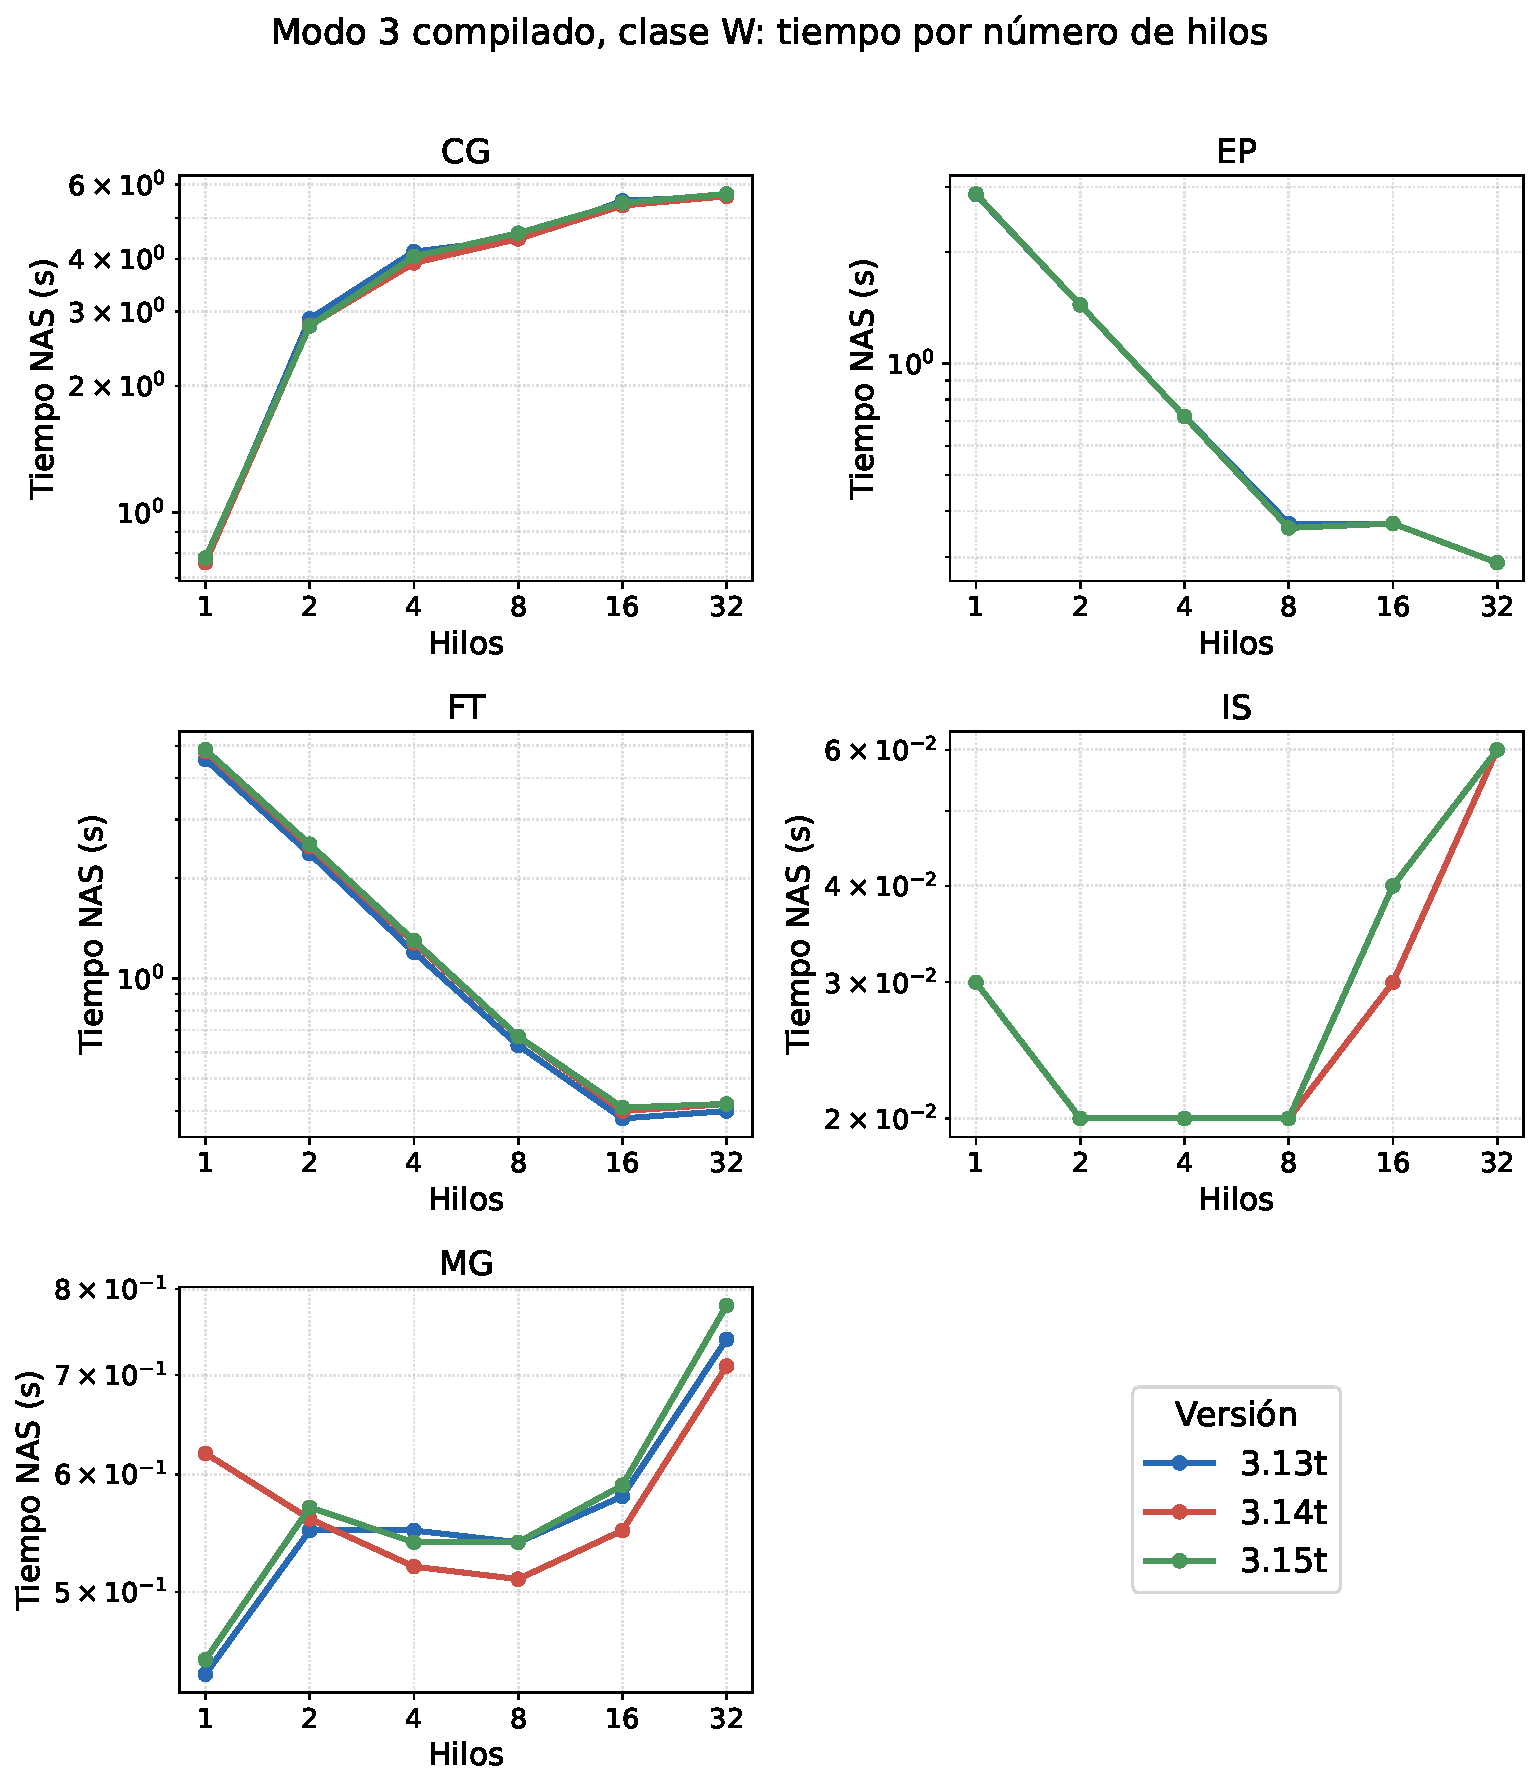
\includegraphics[width=0.92\textwidth]{imagenes/versiones/compilado_tiempos_versiones}
\caption{Tiempo NAS por número de hilos en modo~3 compilado, clase~W, para
Python~3.13t, 3.14t y 3.15t. Las tres versiones se superponen en todos los
benchmarks, en claro contraste con la divergencia del modo interpretado
(Figura~\ref{fig:versiones-interpretado}).}
\label{fig:versiones-compilado}
\end{figure}

Ya en modo~3, las tres versiones se comportan igual en todo el rango de hilos. La
Figura~\ref{fig:versiones-compilado} sigue el tiempo NAS por número de hilos en
cada benchmark, y las tres curvas se superponen casi exactamente. Sea cual sea la
forma de la curva, la fija la estructura del kernel y no la versión del
intérprete. El Anexo~\ref{anexo:tablas-versiones} recoge los tiempos y speedups
completos por número de hilos, los óptimos de cada combinación y las curvas por
benchmark\footnote{Los tiempos absolutos de esta campaña pueden
diferir ligeramente de los del Capítulo~\ref{chap:resultados} para la misma
combinación. Son campañas independientes y la diferencia refleja la variabilidad
entre ejecuciones del clúster.}


\newpage
\section{Conclusiones}
\label{sec:versiones-conclusiones}

La comparación entre versiones tiene dos caras. En los modos compilados, que son
los que dan tiempos prácticos, el comportamiento final no depende de la versión.
Con la afinidad corregida, Python~3.13t, 3.14t y 3.15t mantienen las mismas
conclusiones cualitativas, con EP y FT escalando y CG, IS y MG sin escalabilidad
sostenida. En los modos interpretados, en cambio, la versión sí importa mucho.
Python~3.13t escala bastante peor al aumentar los hilos en CG, FT, IS y MG, y solo
EP queda al margen. Esa penalización se anula al tipar. Donde la versión influye,
Python~3.15t es siempre la más rápida o queda a la par. Las diferencias prácticas
del trabajo están en el modo de ejecución, la estructura del benchmark y la
configuración del runtime.
